\section{Empirical Results}
\subsection{RQ1: Failure Localization}
To answer RQ1, we first examine the distribution of externally observable symptoms across the six inference engines. We then locate the faulty code in nine architectural layers and analyze the association between symptoms and architectural layers. When a bug spans multiple architectural layers, its unit weight is divided equally among those layers so that each bug contributes a total weight of one.
\newcommand{\findbox}[2][]{%
  \noindent
  \begin{tcolorbox}[
    arc=2pt,
    boxrule=0.4pt,
    colback=white,
    colframe=black,
    left=1mm,
    right=1mm,
    top=0.8mm,
    bottom=0.8mm,
    width=\linewidth,
    before skip=2pt,
    after skip=2pt,
    fontupper=\normalsize,
    #1,
  ]
  #2
  \end{tcolorbox}
  \par
}

\begin{figure}[!b]
    \centering
    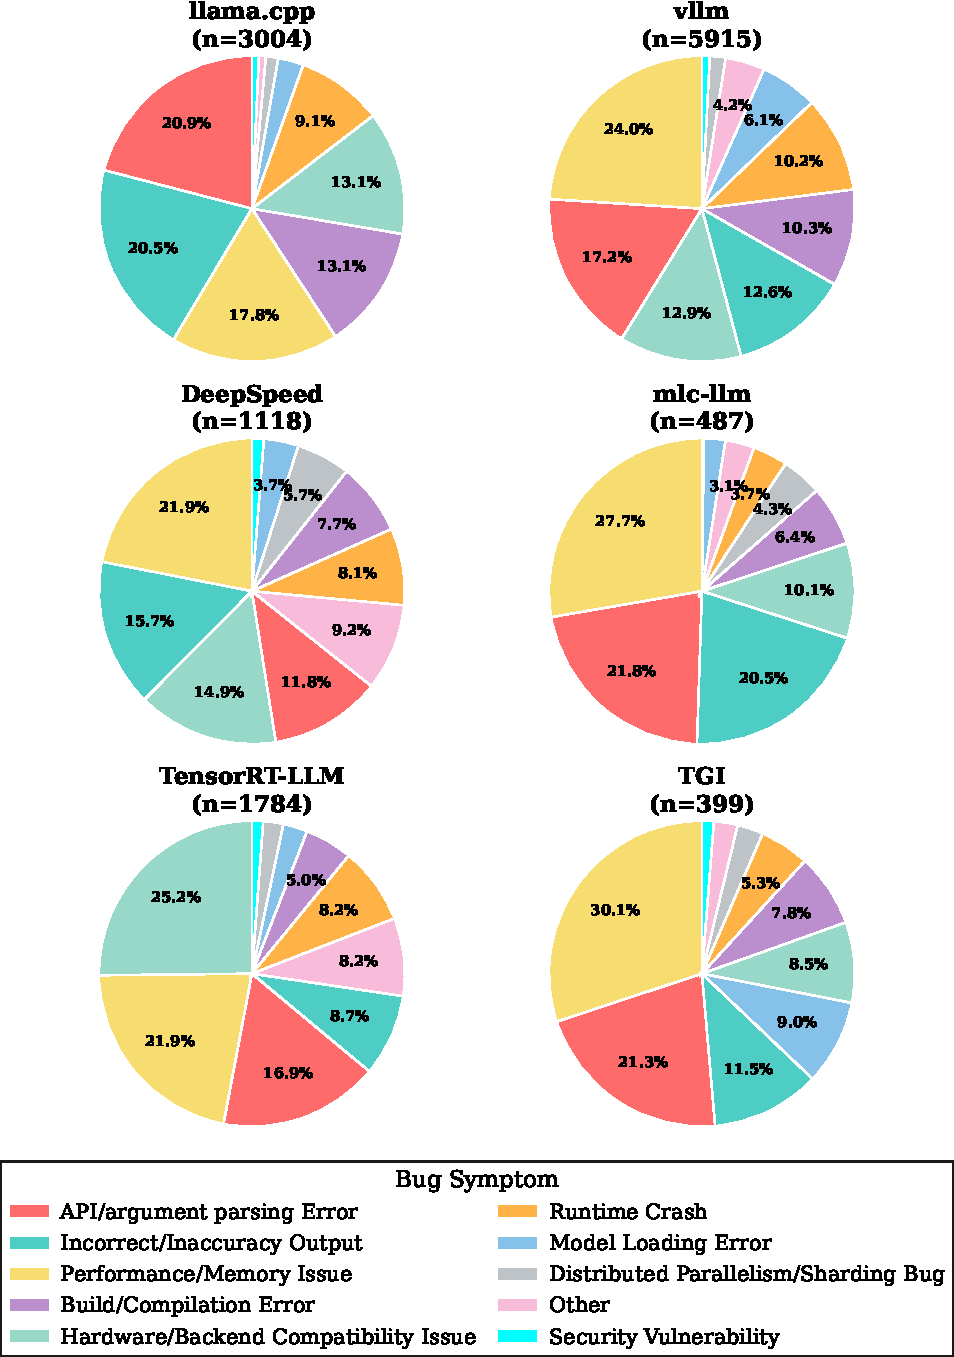
\includegraphics[width=\linewidth]{fig/symptom_distribution_by_project.pdf}
    \caption{Bug-symptom distributions across six inference engines.}
    \label{fig:symptom_dist}
\end{figure}
% \noindent\hspace*{2em}

\noindent\textbf{Observable Symptom Analysis.} As shown in Fig.~\ref{fig:symptom_dist}, we compare how bugs become externally visible across the six inference engines. Together, these distributions reveal which failure manifestations dominate among the studied fixes and which symptoms deserve greater attention in testing.

% \textbf{Critical correctness and availability failures remain common.}
% Figure~\ref{fig:symptom_dist} reveals two common properties of the symptom distributions. 
First, symptoms that threaten correctness and availability constitute a substantial portion of the maintenance burden. Incorrect outputs, runtime crashes, and model-loading failures collectively account for 4,001 of the 12,707 studied bugs (31.5\%), ranging from 23.6\% to 35.6\% across individual engines. This recurring presence matters because the three symptoms expose different detection challenges. Crashes and loading failures usually provide explicit failure signals, whereas incorrect outputs may pass through the serving pipeline without an obvious error. Bug detection should therefore combine conventional crash and initialization checks with output oracles, differential testing, and validation of intermediate execution states. For developers, the result also suggests that regression suites should exercise the complete path from model loading to execution and output validation rather than treating successful startup or request completion as proof of correctness.


% \noindent\hspace*{2em}\textbf{A few symptoms dominate each engine.}
Second, the overall symptom distribution is consistently top-heavy: each engine's three most frequent symptoms account for 52.5\%--70.0\% of its bugs. Because this concentration appears in every project, it is unlikely to be merely an artifact of the largest repositories. The result provides a practical basis for prioritization: project-specific tests, monitors, and bug triage rules targeting a small set of recurrent symptoms can cover a substantial share of historically observed failures. However, the variation in both concentration strength and symptom composition cautions against adopting one global testing profile for all engines. Teams should derive priorities from their own engine's failure history and retain broader checks for the long tail, since even the most concentrated project leaves 30.0\% of bugs outside its top three categories.


% \noindent\hspace*{2em}\textbf{The dominant symptom differs with project emphasis.}
API/argument-parsing errors form the largest category in four engines. They account for 24.0\% of vLLM bugs and 21.9\% of those in DeepSpeed. The corresponding shares rise to 27.7\% in MLC-LLM and 30.1\% in TGI. A different pattern appears in the other two projects. Incorrect outputs lead in llama.cpp and represent 20.9\% of its bugs, whereas 25.2\% of TensorRT-LLM bugs concern performance or memory, making this its most frequent symptom. These profiles are consistent with the different technical surfaces exposed by the projects. Server-oriented engines maintain extensive APIs and configuration paths, llama.cpp emphasizes portable inference across models and platforms, and TensorRT-LLM aggressively targets hardware-specific throughput and memory efficiency. This interpretation explains a plausible correspondence between project emphasis and observed symptoms, but the descriptive data do not establish a causal relationship.
% Finding #1
\findbox{\textbf{Finding \#1:} Bug symptoms concentrate in a few categories across all six engines, but the leading categories differ by project. Incorrect outputs, runtime crashes, and model-loading failures together account for 31.5\% of the corpus; each project's three most frequent symptoms cover 52.5\%--70.0\% of its bugs.}

\begin{figure}[htbp]          % 去掉 *，改为单栏 figure
    \centering
    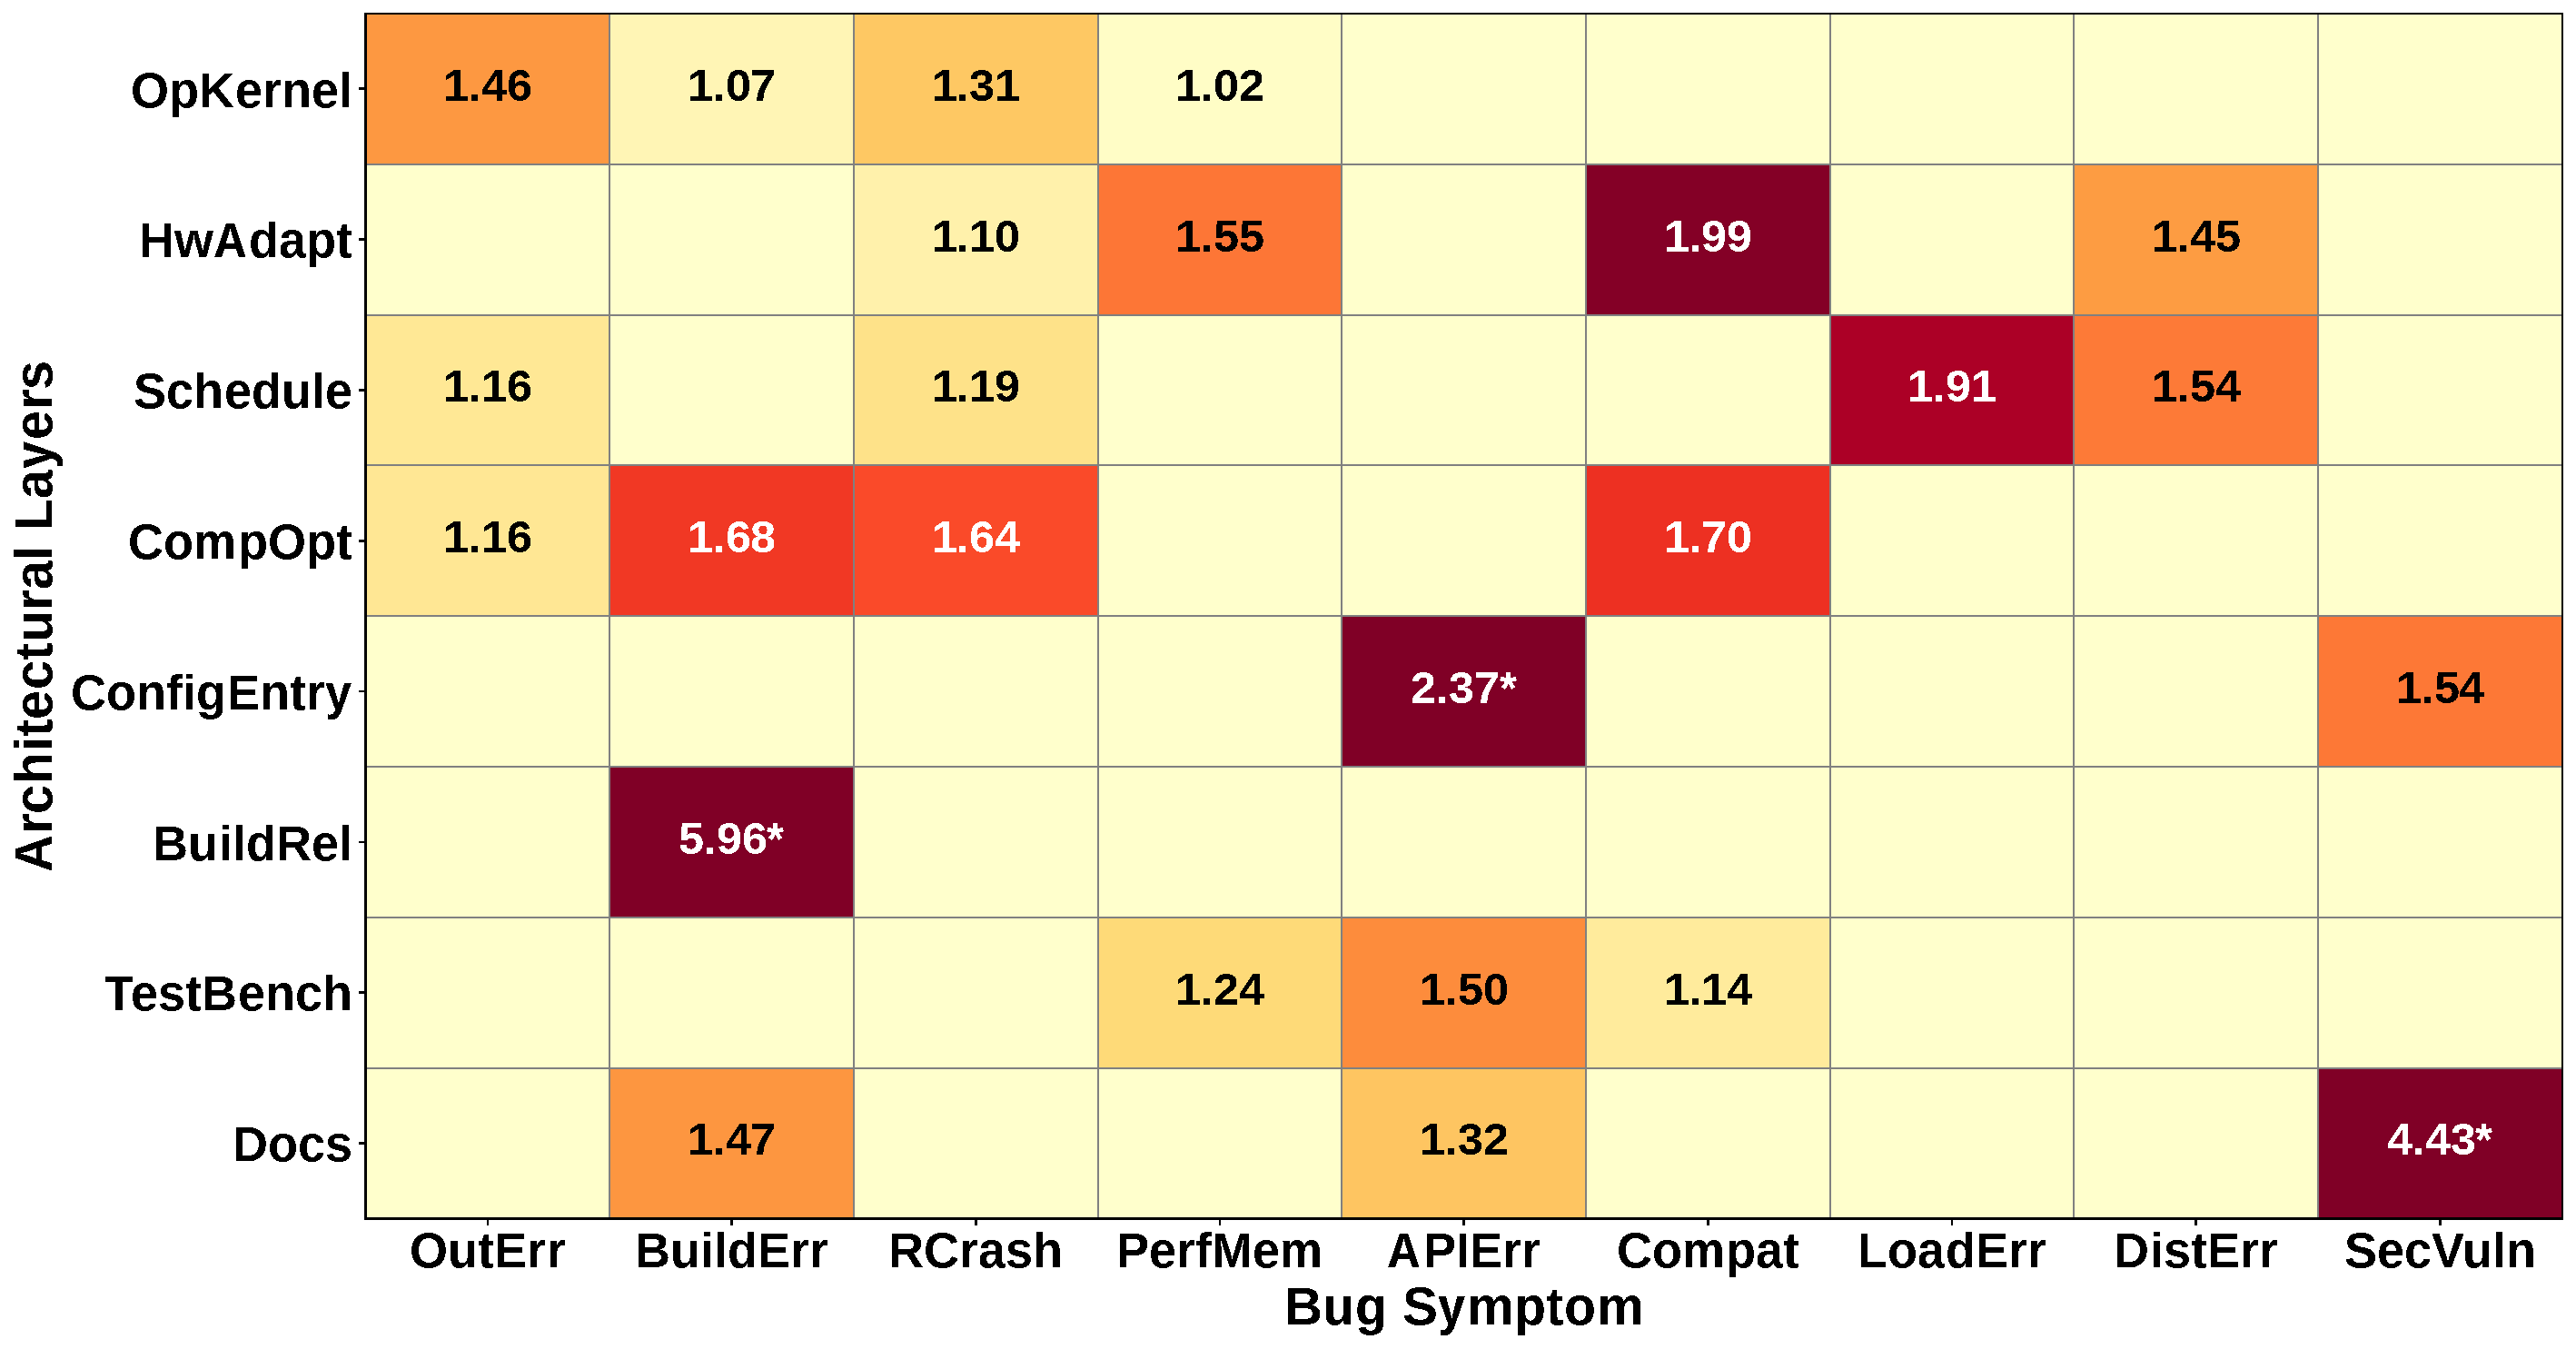
\includegraphics[width=0.95\columnwidth]{fig/root_cause_symptom_lift_heatmap_range_1_2.pdf}
    \caption{Lift of associations between architectural layers and bug symptoms across six LLM inference engines. Values above one mean that a symptom appears more often in a layer than in the full corpus.}
    \label{fig:symptom_arch_layer_lift_heatmap}
\end{figure}
\noindent\textbf{Bug Symptoms Across Architectural Layers.}
Figures~\ref{fig:symptom_arch_layer_lift_heatmap} and~\ref{fig:symptom_distribution_by_arch_layer} expose a markedly uneven relationship between symptoms and architectural layers. Relating the two dimensions reveals which symptoms are more strongly associated with particular architectural layers. Rather than sharing a common symptom distribution, several specialized layers exhibit a distinctive failure signature consistent with their role.


Bugs in Build/Release and Config/Entrypoint are each dominated by one symptom category. Build and compilation errors represent 86.1\% of the weighted bugs in Build/Release and yield the highest observed lift of 5.96. API and argument parsing errors make up 53.0\% of Config/Entrypoint bugs. This symptom is 2.37 times as common in Config/Entrypoint as it is across the full corpus. These profiles give developers focused starting points for diagnosis. Compilation failures direct attention toward dependency specifications, build scripts, and continuous integration environments, while input related failures point toward configuration schemas, request validation, and entrypoint logic. Build matrices and systematic input validation can expose such faults before deployment, while records of resolved configurations can shorten diagnosis when the visible error does not identify its source.

% \noindent\hspace*{2em}\textbf{Hardware Adaptation exposes both compatibility and efficiency problems.}
Hardware Adaptation has a broader symptom profile, yet compatibility and efficiency problems remain prominent. Hardware and backend compatibility issues account for 19.4\% of its weighted bugs and occur at nearly twice the rate expected from the full corpus. Performance and memory issues form an even larger share at 22.6\%. This combination reflects the dual responsibility of hardware specific code, which must preserve functional interoperability while using devices efficiently. Testing this layer should therefore vary devices, drivers, and precision settings while checking both output correctness and resource behavior. Taken together, the three specialized layers show that architectural responsibility influences how faults become visible. Their characteristic symptoms can narrow the initial search area, although they should guide diagnosis rather than determine it.




\begin{figure}[htbp]          % 去掉 *，改为单栏 figure
    \centering
    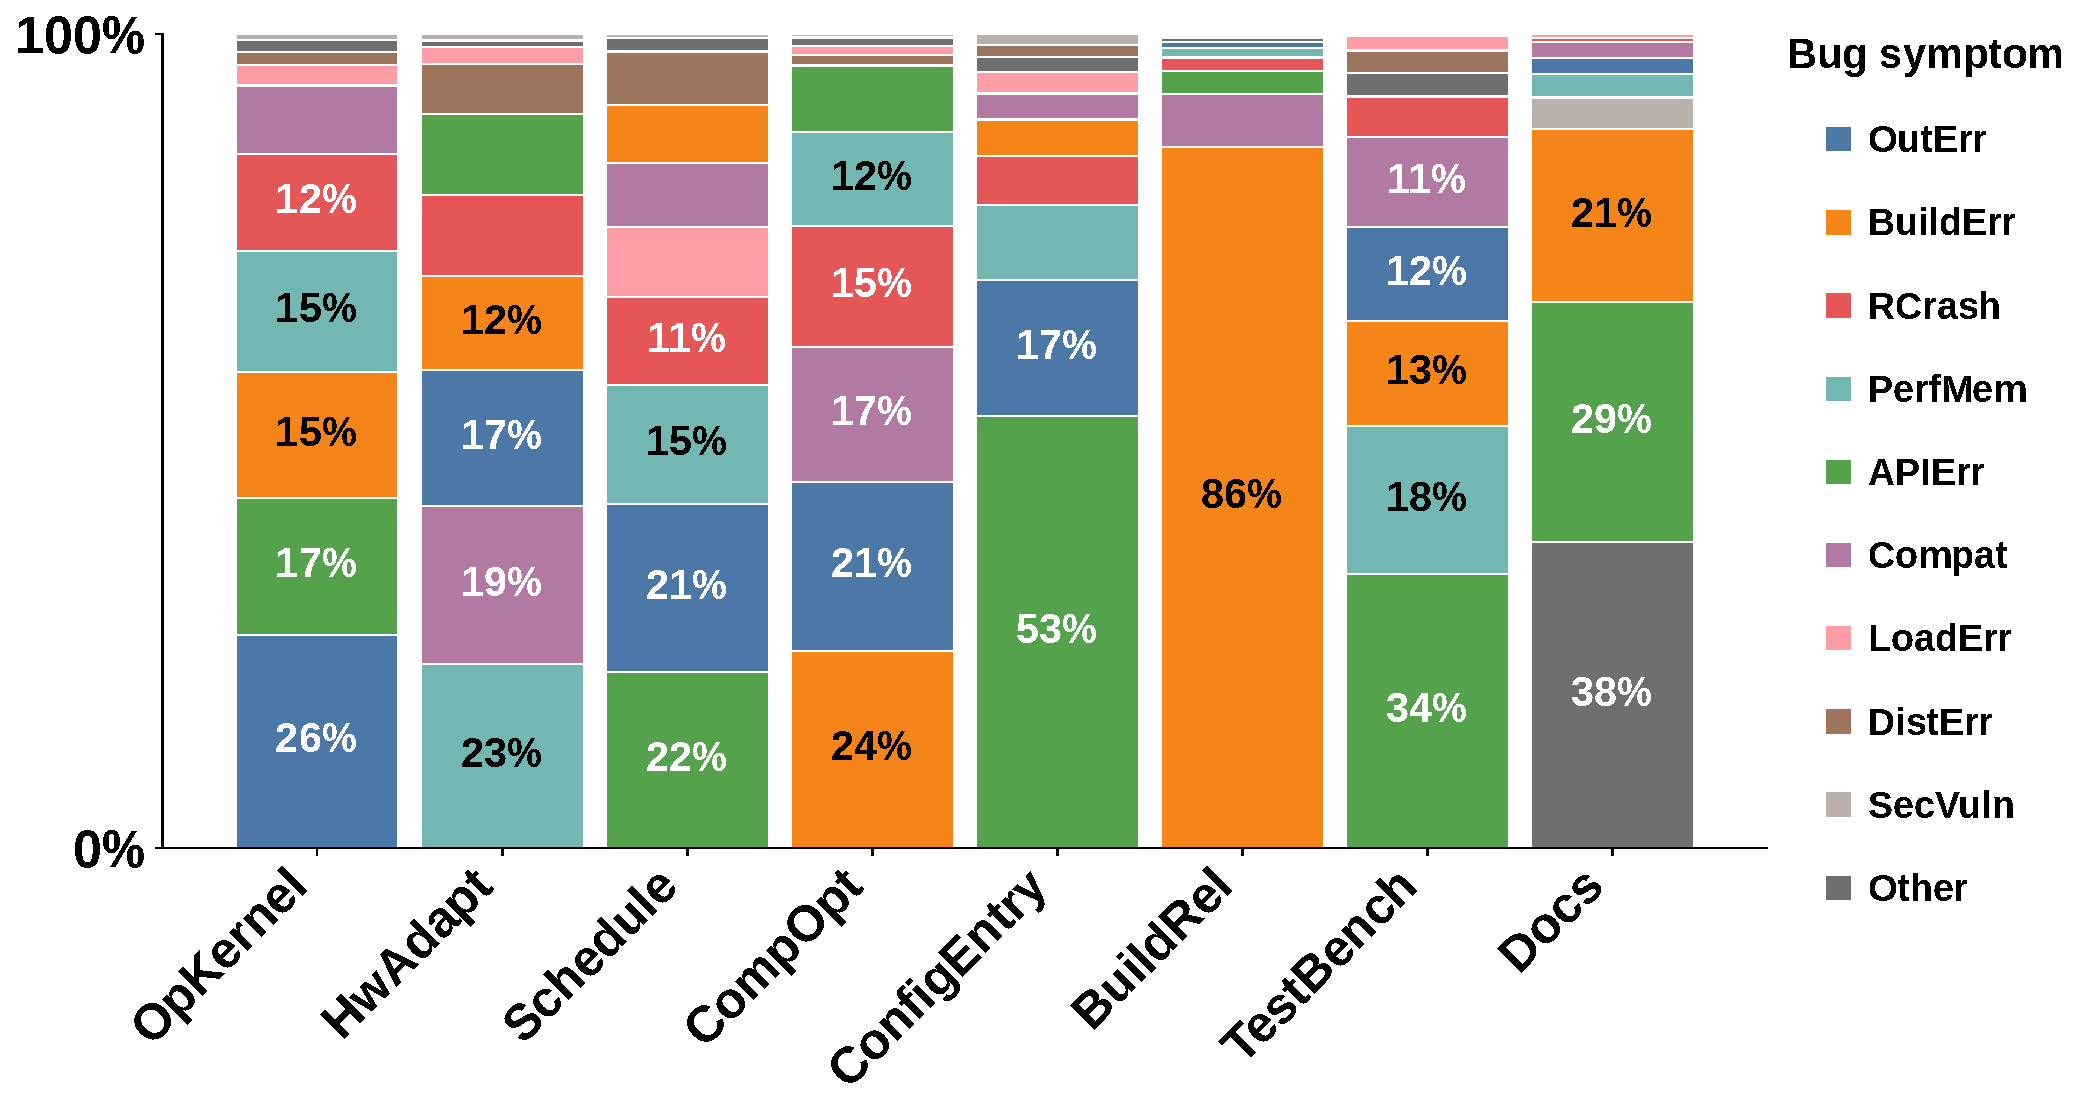
\includegraphics[width=0.95\columnwidth]{fig/root_cause_symptom_stacked_percentage.pdf}
    \caption{Distribution of bug symptoms within each architectural layer across six LLM inference engines.}
    \label{fig:symptom_distribution_by_arch_layer}
\end{figure}
% Finding #2
\findbox[before skip=6pt,after skip=0pt]{\textbf{Finding \#2:} Symptom profiles vary systematically across architectural layers. In particular, Build/Release, Config/Entrypoint, and Hardware Adaptation exhibit narrow failure signatures aligned with their roles, so their characteristic symptoms can guide initial localization.}

% \noindent\textbf{}

Scheduler/Runtime illustrates why a frequent layer is not necessarily easy to diagnose. It contains 38.5\% of the weighted bugs, yet no symptom accounts for one quarter of them. API and argument parsing errors lead at only 21.6\%, closely followed by incorrect outputs at 20.7\%. The remaining failures include performance problems, crashes, and failures involving loading or distributed execution. This diversity is consistent with the coordinating role of scheduler and runtime code. A single request may depend on admission and batching, model and memory state, and distributed worker execution before producing a result. Faults in any of these interactions can therefore converge on similar external symptoms. Monitoring only final outcomes provides little evidence about where the failure began. Developers need stage level telemetry that records queue transitions, cache state, and distributed worker events across the request lifetime.

Compiler/Optimization accounts for only 3.4\% of the weighted corpus but shows a similarly broad profile. Build and compilation errors form its largest category at 24.2\%, while incorrect outputs follow closely at 20.8\%. Another 16.6\% appear as hardware or backend compatibility problems. These outcomes show that an optimization fault does not always stop compilation. An invalid transformation may instead generate a numerically incorrect kernel, fail only on a particular backend, or alter runtime resource use. A successful build is therefore a weak oracle for this layer. Tests should compare optimized and unoptimized execution, inspect intermediate representations, and validate results across backend and precision settings.

The contrast with Finding~\#2 lies in diagnostic specificity rather than bug frequency alone. A build or parsing error can substantially narrow the likely search area. Crashes, incorrect outputs, and performance regressions provide weaker guidance because several interacting execution layers can produce them. Effective diagnosis in Scheduler/Runtime and Compiler/Optimization must connect the final symptom with runtime traces, intermediate states, and backend comparisons. Tests that span model preparation, request execution, and device execution are also needed to reveal failures that emerge only through cross layer interactions.

% Finding #3
\findbox{\textbf{Finding \#3:} In contrast to specialized boundary layers, Scheduler/Runtime and Compiler/Optimization produce broad, overlapping symptom profiles. Their faults cross correctness, availability, performance, and compatibility boundaries, making symptom-only localization substantially less reliable.}

\begin{table}[t]
    \centering
    \caption{Definitions of repair operations.}
    \label{tab:repair_operations}
    \renewcommand{\arraystretch}{1.3}
    \setlength{\tabcolsep}{3pt}
    \begin{tabular}{p{0.22\columnwidth} p{0.63\columnwidth} c}
        \toprule
        \textbf{Operation} & \multicolumn{1}{c}{\textbf{Description}} & \textbf{ID} \\
        \midrule
        Logic Correction & Fixes logical errors, calculations, conditions, or state transitions. & (Cor) \\
        Adaptation & Adjusts for different hardware, platforms, APIs, or compatibility. & (Adp) \\
        Configuration & Modifies runtime options, default parameters, or feature flags. & (Cf) \\
        Validation & Adds checks to reject invalid inputs, states, permissions, or preconditions. & (Val) \\
        Reorganization & Restructures data structures, control flow, or module interactions. & (Rg) \\
        Recovery & Enhances failure handling, rollbacks, retry, or fallback mechanisms. & (Rv) \\
        Optimization & Improves performance/memory efficiency without behavioral changes. & (Opt) \\
        Synchronization & Adjusts ordering or coordination across threads, devices, or processes. & (S) \\
        Allocation & Changes memory, buffer, cache, or resource allocation and release. & (Al) \\
        \bottomrule
    \end{tabular}
\end{table}

\subsection{RQ2: Repair Structure}

RQ2 examines repair structure through repair operations, code entity concentration, and fix scope. Each fix is assigned one of the nine repair operations defined in Table~\ref{tab:repair_operations}. Fifteen fixes with rare residual operations are grouped as Other and excluded from the operation analysis. When a fix spans multiple architectural layers, its operation contributes one instance to each assigned layer. The resulting 19,965 instances describe layer participation rather than unique fixes.

Code entity concentration is measured separately for files and functions. Fix scope is measured with changed lines and modified files, which capture the amount and breadth of code modification. Complete diffs are available for all 12,707 fixes. Since changed lines are strongly skewed, we use the median and upper quantiles instead of the mean. The median is 14 lines, while P75, P90, and P95 reach 52, 165, and 326.7 lines.


\noindent\textbf{Code Entity Concentration.}
The resulting concentration profiles show where bug-fixing activity has historically accumulated and which code entities may warrant closer attention. Figure~\ref{fig:file_function_concentration} shows that bug fixes are concentrated in a limited portion of the codebase. The top 20\% of files account for 79.6\% of weighted bug associations, while the same fraction of functions accounts for 68.4\%. This difference suggests that maintenance repeatedly returns to a small group of modules but spans several implementation units in each. File histories can therefore identify modules that deserve early attention, while function histories provide a finer search space for diagnosis and review.

The pattern persists in every engine rather than being produced by one large repository. Depending on the project, the top 20\% of files cover between 69.3\% and 85.1\% of weighted bug associations. Function coverage ranges from 61.7\% to 69.4\%. These recurring concentrations support a staged quality assurance strategy. Teams can use file histories to prioritize risky modules, then use function histories to focus regression testing, review, and refactoring.

\findbox{\textbf{Finding \#4:} Bugs are strongly concentrated in a small set of files and functions. The top 20\% of files account for 79.6\% of weighted bug associations, while the top 20\% of functions account for 68.4\%.}

\begin{figure}[t]
    \centering
    \subfloat{%
        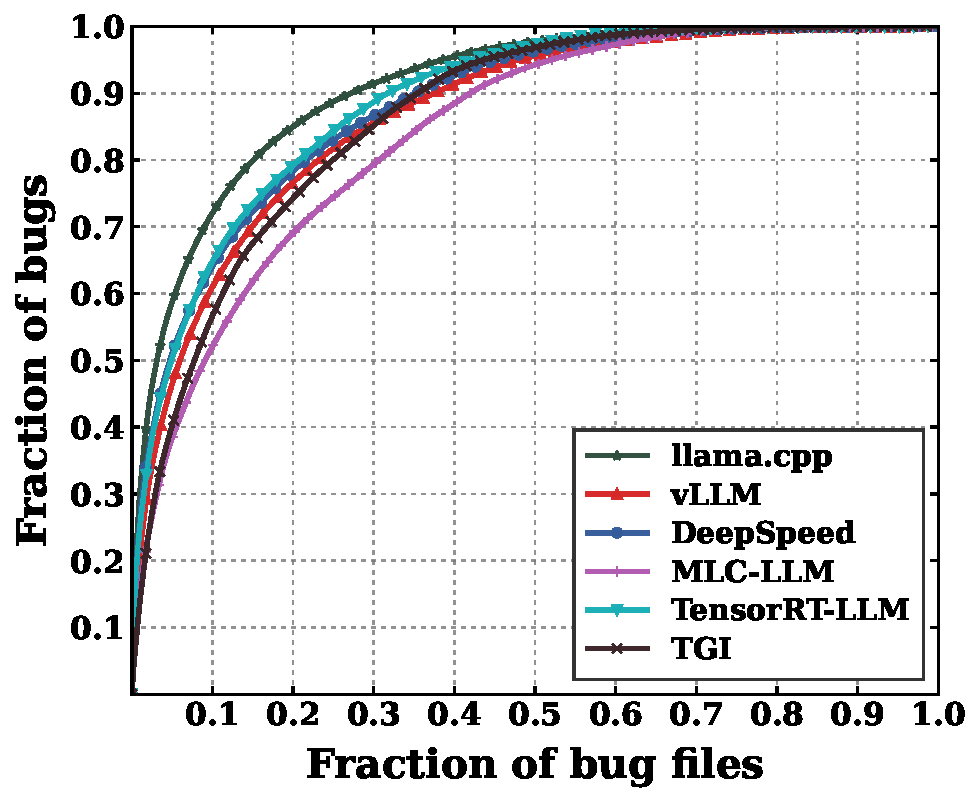
\includegraphics[width=0.49\columnwidth]{fig/concentration_curve_files_weighted_alpha0.8_by_project_multi_project.pdf}%
    }\hfill
    \subfloat{%
        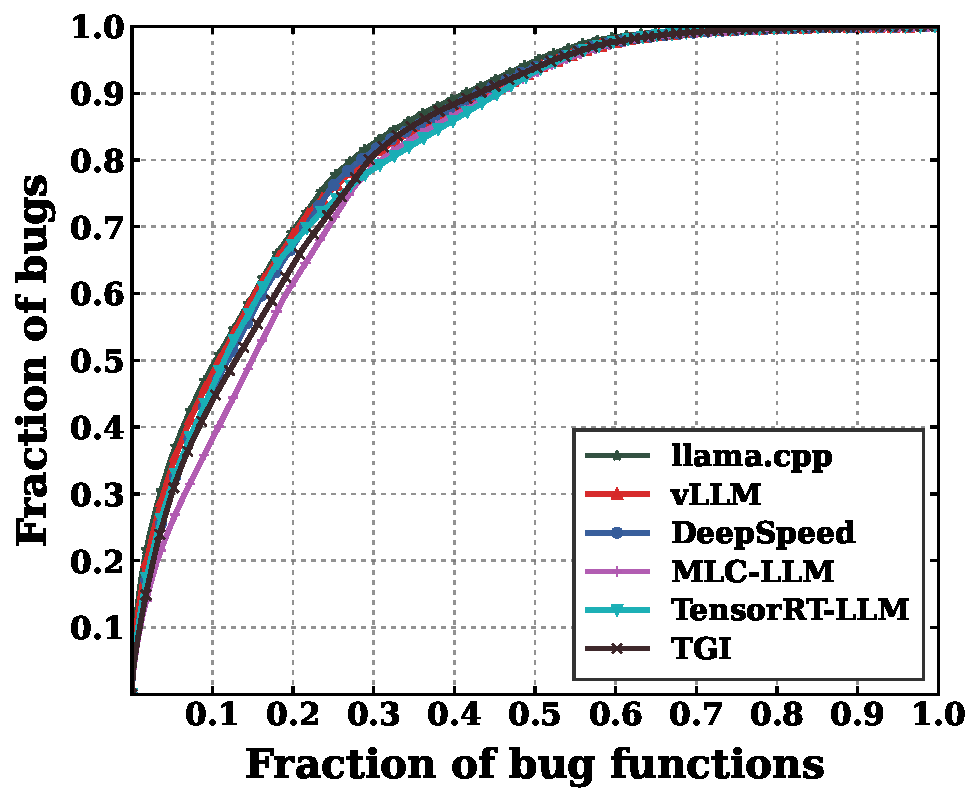
\includegraphics[width=0.49\columnwidth]{fig/concentration_curve_functions_weighted_alpha0.8_by_project_multi_project.pdf}%
    }
    \caption{Per-project bug concentration curves at file and function granularity. Entities are ranked in descending order by their associated bug counts. The x-axis represents the cumulative fraction of files or functions, and the y-axis represents the cumulative fraction of bugs.}
    \label{fig:file_function_concentration}
\end{figure}

\noindent\textbf{Repair Operation Distribution.}
Examining this distribution reveals which forms of code change dominate maintenance and how their prevalence varies across architectural layers. Table~\ref{tab:repair_counts} shows that Logic Correction and Adaptation account for 14,702 of the 19,965 repair operation instances, or 73.6\%. Their dominance shows that much of the maintenance workload addresses faulty program behavior or adapts the engine to changing execution environments. Review and testing should therefore pay particular attention to state transitions, compatibility assumptions, and behavior across supported platforms. The concentration also suggests that repair tools designed around these recurring operations could assist a substantial portion of observed fixes without assuming that all layers fail in the same way.

The two operations remain prevalent across most of the architecture. Their combined share exceeds 65\% in seven of the eight principal layers and reaches 80.5\% in Compiler/Optimization. Build/Release is the exception. Logic Correction and Adaptation account for 46.7\% of its instances, while Configuration alone contributes 43.2\%. This distinct profile reflects the role of build scripts, dependency specifications, and packaging settings. It also indicates that maintenance support for this layer should emphasize configuration validation rather than relying only on techniques aimed at program logic or platform adaptation.

\findbox{\textbf{Finding \#5:} Repair operations exhibit a highly concentrated distribution. Logic Correction and Adaptation dominate the overall maintenance workload and remain prevalent across most architectural layers.}

\begin{table}[t]
    \centering
    \caption{Architectural layer \(\times\) repair operation counts.}
    \label{tab:repair_counts}
    \resizebox{\linewidth}{!}{%
        \begin{tabular}{l c c c c c c c c c}
            \toprule
            \diagbox[width=2.4cm, height=0.6cm]{\textbf{Layer}}{\raisebox{0pt}{\hspace{1.25cm}\textbf{Operation}}}
            & \textbf{Corr.} & \textbf{Adapt.} & \textbf{Config.} & \textbf{Valid.} & \textbf{Reorg.} & \textbf{Recov.} & \textbf{Optim.} & \textbf{Sync.} & \textbf{Alloc.} \\[-0.18cm]
            & (Cor) & (Adp) & (Cf) & (Val) & (Rg) & (Rv) & (Opt) & (S) & (Al) \\[+0cm]
            \midrule
            Scheduler/Runtime & 3816 & 2305 & 239 & 515 & 450 & 228 & 228 & 163 & 35 \\
            Hardware Adapt. & 1477 & 1495 & 126 & 179 & 182 & 131 & 123 & 123 & 81 \\
            Operators/Backend & 1279 & 746 & 81 & 206 & 147 & 69 & 67 & 38 & 43 \\
            Config/Entrypoint & 896 & 442 & 187 & 231 & 158 & 61 & 29 & 29 & 6 \\
            Tests/Bench & 648 & 560 & 321 & 111 & 87 & 67 & 11 & 25 & 9 \\
            Compiler/Optim. & 314 & 267 & 29 & 31 & 17 & 10 & 39 & 11 & 4 \\
            Build/Release & 102 & 143 & 227 & 15 & 31 & 5 & 0 & 2 & 0 \\
            Docs & 196 & 16 & 53 & 1 & 0 & 2 & 0 & 0 & 0 \\
            \bottomrule
        \end{tabular}%
    }
\end{table}



\subsection{RQ3: Repair Evolution}
For RQ3, we track how bug-fixing activity changes over time in both repair scope and architectural distribution. The analysis includes 12,707 pull requests with complete diffs and valid timestamps from February 2020 to March 2026. Monthly observations are sparse during the early development of several projects, so the formal trend analysis covers the 12,299 fixes created between January 2023 and March 2026.

Modified files measure how broadly a fix spreads across the codebase. To examine whether the architectural focus of bug-fixing activity also changes, we compute the monthly weighted share of each architectural layer. Following RQ1, the layers assigned to a bug are first deduplicated, and a bug spanning $k$ layers contributes $1/k$ to each layer so that every bug has a total weight of one. We use Spearman's rank correlation to assess monotonic trends over the 39 monthly observations and apply the Benjamini--Hochberg procedure across the nine layer-level tests. Each observation is assigned to the creation month of its fixing pull request. The results therefore describe the evolution of observed bug-fixing activity rather than bug introduction time, discovery delay, or changes in the intrinsic reliability of an architectural layer.

\begin{figure}[t]
    \centering
    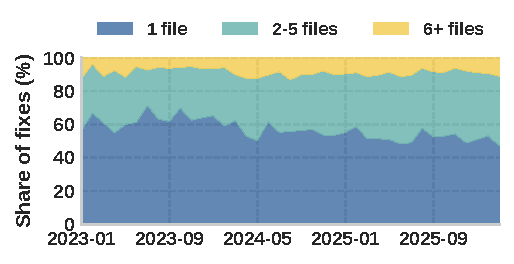
\includegraphics[width=\columnwidth]
        {fig/monthly_file_bucket_trend_single_column.pdf}
    \caption{Monthly distribution of bug fixes by the number of modified files from January 2023 to March 2026.}
    \label{fig:monthly-file-bucket-trend}
\end{figure}

\noindent\textbf{File Breadth Evolution.}
Tracking file breadth clarifies how widely fixes spread and whether repairs increasingly involve coordinated changes across multiple files. Figure~\ref{fig:monthly-file-bucket-trend} shows that single file fixes remain the largest category, but their share decreases from 56.3\% in January 2023 to 47.1\% in March 2026. Over the same period, fixes spanning two to five files rise from 31.3\% to 41.8\%. The similar size of these changes indicates that the main shift occurs from isolated modifications toward repairs requiring coordination across a small group of files. Developers should review connected changes together and test interactions among the modified components.

Fixes touching at least six files grow from 4 to 95 in monthly volume, yet their share changes from 12.5\% to 11.1\%. Their absolute workload increases as project activity expands, but they do not become more prevalent relative to other fixes. The evidence therefore indicates a broader routine repair surface, not a growing proportion of very large multi-file changes.

% Finding #6
\findbox{\textbf{Finding \#6:} Single-file fixes remain the largest category, but the repair mix shifts toward changes spanning two to five files. Fixes touching six or more files grow strongly in absolute volume without increasing their relative share.}

\begin{table}[t]
    \centering
    \caption{Weighted architectural-layer changes over time.}
    \label{tab:monthly-layer-trends}
    \scriptsize
    \setlength{\tabcolsep}{3pt}
    \resizebox{\columnwidth}{!}{%
    \begin{tabular}{lrrrrr}
        \toprule
        \textbf{Architectural layer} &
        \textbf{First 12m} &
        \textbf{Last 12m} &
        \boldmath$\Delta$ \textbf{(pp)} &
        \boldmath$\rho$ &
        \boldmath$\rho_{\mathrm{adj}}$ \\
        \midrule
        Hardware Adaptation      &  6.4\% & 23.7\% & $+17.2$ &  $0.781$ &  $0.739$ \\
        Tests/Bench              &  3.2\% & 12.5\% &  $+9.3$ &  $0.822$ &  $0.675$ \\
        Config/Entrypoint        &  4.9\% & 10.4\% &  $+5.5$ &  $0.564$ &  $0.239$ \\
        Compiler/Optimization    &  2.1\% &  4.0\% &  $+2.0$ &  $0.525$ &  $0.443$ \\
        \midrule
        Scheduler/Runtime        & 44.1\% & 33.6\% & $-10.5$ & $-0.382$ & $-0.668$ \\
        Docs                     &  2.8\% &  1.1\% &  $-1.7$ & $-0.576$ & $-0.154$ \\
        Operators/Backend        & 22.4\% &  9.1\% & $-13.3$ & $-0.654$ & $-0.156$ \\
        Other                    &  6.8\% &  3.7\% &  $-3.1$ & $-0.670$ & $-0.137$ \\
        Build/Release            &  7.2\% &  1.9\% &  $-5.3$ & $-0.789$ & $-0.645$ \\
        \bottomrule
    \end{tabular}
    }
    \vspace{2pt}

    \begin{minipage}{\columnwidth}
        \scriptsize
        \emph{Notes:} ``First'' and ``Last'' are mean monthly shares; $\Delta$ is their difference in percentage points. $\rho$ is the pooled Spearman correlation and $\rho_{\mathrm{adj}}$ uses fixed project weights. Here, $q$ denotes the Benjamini--Hochberg-adjusted $p$-value. All pooled trends remain significant after correction ($q\leq0.0011$), except Scheduler/Runtime ($q=0.017$).
    \end{minipage}
\end{table}

\noindent\textbf{Architectural Composition Evolution.}
The layer trends in Table~\ref{tab:monthly-layer-trends} show that the architectural distribution of bug-fixing activity changes substantially over the study period. Hardware Adaptation exhibits the clearest increase. Its monthly weighted share has a strong positive association with time ($\rho=0.781$, $p<0.001$), rising from an average of 6.4\% during the first 12 months of the analysis window to 23.7\% during the last 12 months. This difference of 17.2 percentage points is also reflected in an estimated increase of 7.3 percentage points per year. After correcting for the nine layer-level comparisons, the trend remains statistically significant ($q<0.001$).

This result is not explained solely by the changing contribution of the six projects. A project-standardized monthly series, constructed using fixed analysis-window project weights, retains a strong positive association ($\rho=0.739$) and an estimated increase of 6.6 percentage points per year. The direction is also positive within several engines, with particularly clear increases in llama.cpp, TGI, and vLLM. Together, these observations indicate that the growing share of Hardware Adaptation fixes reflects a recurring cross-project shift rather than only the expansion of one repository.

Tests/Bench also increases in the pooled data ($\rho=0.822$, $p<0.001$), from 3.2\% in the first 12 months to 12.5\% in the last 12 months. Unlike Hardware Adaptation, however, this pattern is driven primarily by vLLM and is nearly flat in most other projects. We therefore treat it as a project-dependent trend rather than evidence of a common architectural shift across inference engines.

Because the monthly layer shares sum to 100\%, these trends describe a change in composition. An increase in one layer necessarily coincides with decreases elsewhere, and a larger share of fixes does not establish that the layer itself became less reliable. Nevertheless, the persistent and cross-project rise of Hardware Adaptation suggests that compatibility with heterogeneous accelerators and execution backends occupies an increasingly prominent place in inference-engine maintenance. This implication motivates closer attention to backend-specific validation, while the observational evidence does not identify the technical or organizational causes of the shift.

\findbox{\textbf{Finding \#7:} Bug-fixing activity increasingly shifts toward Hardware Adaptation. Its weighted share rises strongly over time; the trend persists after accounting for project composition and appears across multiple engines.}
